\documentclass[10pt]{article}
\usepackage[a4paper,margin=0.75in]{geometry}
\usepackage{amsmath,amssymb}
\usepackage{graphicx}
\usepackage[hidelinks]{hyperref}

% figure roots: raw paper crops, and our solo/composite renders
\graphicspath{{../references/paper_figures/}{../reports/collaborator_2026-06/figures_solo/}}

\pagestyle{empty}
\setlength{\parindent}{0pt}
\setlength{\parskip}{0pt}

\newcommand{\arxiv}[1]{\href{https://arxiv.org/abs/#1}{\texttt{arXiv:#1}}}
\newcommand{\hepph}[1]{\href{https://arxiv.org/abs/hep-ph/#1}{\texttt{hep-ph/#1}}}

% section header: bold label over a full-width rule
\newcommand{\sechead}[1]{%
  \vspace{0.9em}{\large\bfseries #1}\par\vspace{2pt}\hrule height 0.7pt\vspace{0.6em}}

% entry header: title, authors, internal tag, arXiv id(s)
\newcommand{\hdr}[4]{%
  \vspace{12pt}
  {\large\bfseries #1}\par\vspace{1pt}
  {\small #2\ \ (#3)\hfill #4}\par\vspace{3pt}\hrule\vspace{6pt}}

% trailing equation-number tag
\newcommand{\eqn}[1]{\hfill{\footnotesize (#1)}}

\begin{document}

\begin{center}
{\Large\bfseries Custodial implementation: reference map}\\[3pt]
{\normalsize The equation each formula comes from, and the figure each paper computes.}
\end{center}
\vspace{0.15em}
\hrule height 0.8pt
\vspace{0.4em}
{\footnotesize Notation: $L=k\pi r_c\approx35$ (warped volume); $M_{KK}$ first KK mass; $v\approx174$~GeV; $x_1\approx2.45$ (first gauge-KK root); $B_d,B_Q$ flavour-sum factors (CGHNP); $s=\sin\theta_W$, $c_W=\cos\theta_W$.}

\sechead{Formula sources}

% ---------------- CGHNP ----------------
\hdr{Flavor Physics in the Randall-Sundrum Model, I}
    {Casagrande, Goertz, Haisch, Neubert, Pfoh}{CGHNP}{\arxiv{0807.4937}}
\noindent
\begin{minipage}[t]{0.55\textwidth}
{\small\itshape Formulas taken}\\[4pt]
{\small
$\displaystyle \Delta T_{\min}=\frac{\pi v^2}{2c_W^2 M_{KK}^2}\!\left(L-\tfrac{1}{2L}\right)$\eqn{Eq.~147}\\[7pt]
$\displaystyle \Delta T_{\mathrm{cust}}=-\frac{\pi v^2}{4c_W^2 M_{KK}^2}\,\frac{1}{L}$\eqn{Eq.~153, after ADMS}\\[7pt]
$\displaystyle \delta g_L^b=+\frac{m_b^2}{2M_{KK}^2}B_d,\ \ \delta g_R^b=-\frac{m_b^2}{2M_{KK}^2}B_Q$\eqn{Eq.~170}
}
\end{minipage}\hfill
\begin{minipage}[t]{0.42\textwidth}
\centering
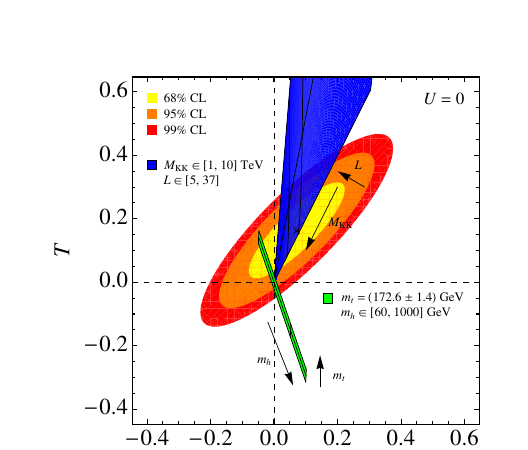
\includegraphics[width=\linewidth]{casagrande_fig4_ST.png}\\[2pt]
{\footnotesize Fig.~4: minimal-RS $S$--$T$ wedge, the volume-enhanced $T$ that custodial SU(2)$_R$ then protects.}
\end{minipage}

% ---------------- ADMS ----------------
\hdr{RS1, Custodial Isospin and Precision Tests}
    {Agashe, Delgado, May, Sundrum}{ADMS}{\hepph{0308036}}
\noindent
\begin{minipage}[t]{0.55\textwidth}
{\small\itshape Formula taken (mechanism)}\\[4pt]
{\small
No closed form is copied. SU(2)$_R$ removes the $\log(k\pi r_c)$ enhancement of $T$:
\\[6pt]
$\displaystyle T:\ \underbrace{+\tfrac{\pi L}{2c_W^2}}_{\text{minimal}}\ \xrightarrow{\ \mathrm{SU(2)}_R\ }\ \underbrace{-\tfrac{\pi}{4c_W^2 L}}_{\text{custodial}}$\eqn{ADMS Eq.~4.9/5.6}
\\[6pt]
the $+L\to-1/L$ flip that CGHNP distil into Eq.~153.
}
\end{minipage}\hfill
\begin{minipage}[t]{0.42\textwidth}
{\small\itshape What the paper computes}\\[4pt]
{\small $T$ (protected, leaving a $\sim\!3$~TeV floor set by $S$), $S$ (unprotected), and $Zb_L$. Analytic paper; no data figure.}
\end{minipage}

% ---------------- ACDP ----------------
\hdr{A Custodial Symmetry for $Z b\bar b$}
    {Agashe, Contino, Da Rold, Pomarol}{ACDP}{\hepph{0605341}}
\noindent
\begin{minipage}[t]{0.55\textwidth}
{\small\itshape Formulas taken}\\[4pt]
{\small
$\displaystyle P_{LR}:\ c_1=c_2\ \Rightarrow\ \delta g_L^b\big|_{\text{tree}}=0,\quad q_L\in(2,2)_{2/3}$\eqn{Eqs.~3--12}\\[7pt]
$\displaystyle b_R\in(1,1)_{-1/3}:\ T^3_L=T^3_R=0\ \Rightarrow\ \delta g_R^b=0\ (P_C)$\eqn{Eq.~22 / Table~1}
}
\end{minipage}\hfill
\begin{minipage}[t]{0.42\textwidth}
{\small\itshape What the paper computes}\\[4pt]
{\small $\delta g_L^b$ (protected) and the representation-dependent $\delta g_R^b$, custodial versus minimal; the $A_{FB}^b$ anomaly. No data figure (analytic).}
\end{minipage}

% ---------------- CPSW ----------------
\hdr{Light Kaluza-Klein States, and Electroweak Constraints, with Custodial SU(2)}
    {Carena, Pont\'on, Santiago, Wagner}{CPSW}{\hepph{0607106},\ \hepph{0701055}}
\noindent
\begin{minipage}[t]{0.55\textwidth}
{\small\itshape Formulas taken (top-partner one loop)}\\[4pt]
{\small
$\displaystyle \delta g_L^{b,\,\mathrm{singlet}}=\frac{\alpha}{16\pi s^2 M_W^2}\frac{m_{q_0 t}^4}{M_t^2}\,[1+\cdots]$\eqn{Eq.~14}\\[7pt]
$\displaystyle \delta g_L^{b,\,\mathrm{bidoublet}}=\frac{\alpha}{32\pi s^2 M_W^2}\,m_t^2\,[\cdots]$\eqn{Eq.~15}\\[7pt]
$\displaystyle \Delta T_{\mathrm{top}}=T_{\mathrm{top}}\,\frac{2 m_{q_0 t}^2}{M_t^2}\,[\cdots]$\eqn{Eq.~13, $T_{\mathrm{top}}$ from Eq.~35}
}
\end{minipage}\hfill
\begin{minipage}[t]{0.42\textwidth}
\centering
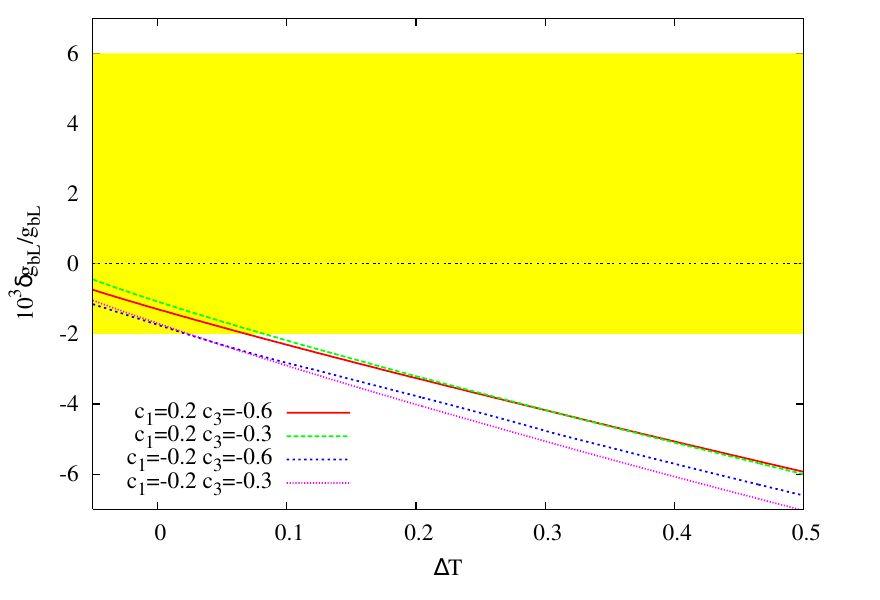
\includegraphics[width=\linewidth]{carena_0701055_fig1_T_dgbL.png}\\[2pt]
{\footnotesize Fig.~1: loop $\delta g_{bL}/g$ vs.\ $\Delta T$. Top partners re-introduce a negative $\delta g_L^b$ correlated with $+\Delta T$ (bidoublet $-T$, singlet $+T$); floor $\sim\!2.5$--$3$~TeV ($S$-set).}
\end{minipage}

\sechead{Comparison and validation (no formulas taken)}

% ---------------- CFW ----------------
\hdr{The Flavor of the Composite Pseudo-Goldstone Higgs}
    {Cs\'aki, Falkowski, Weiler}{CFW}{\arxiv{0804.1954}}
\noindent
\begin{minipage}[t]{0.55\textwidth}
{\small\itshape Formulas taken}\;{\small none.}\\[6pt]
{\small\itshape What the paper computes}\\[4pt]
{\small Anarchic $\varepsilon_K$ from the KK gluon ($\mathrm{Im}\,\Lambda_{LR}$, $s\to d$):
\\[4pt]
$\displaystyle M_{KK}\gtrsim 21~\text{TeV (RS)},\quad 33~\text{TeV (gauge-Higgs)},$
\\[4pt]
with the electroweak sector held near $3$~TeV by custodial. The explicit electroweak-versus-flavor split we reproduce.}
\end{minipage}\hfill
\begin{minipage}[t]{0.42\textwidth}
\centering
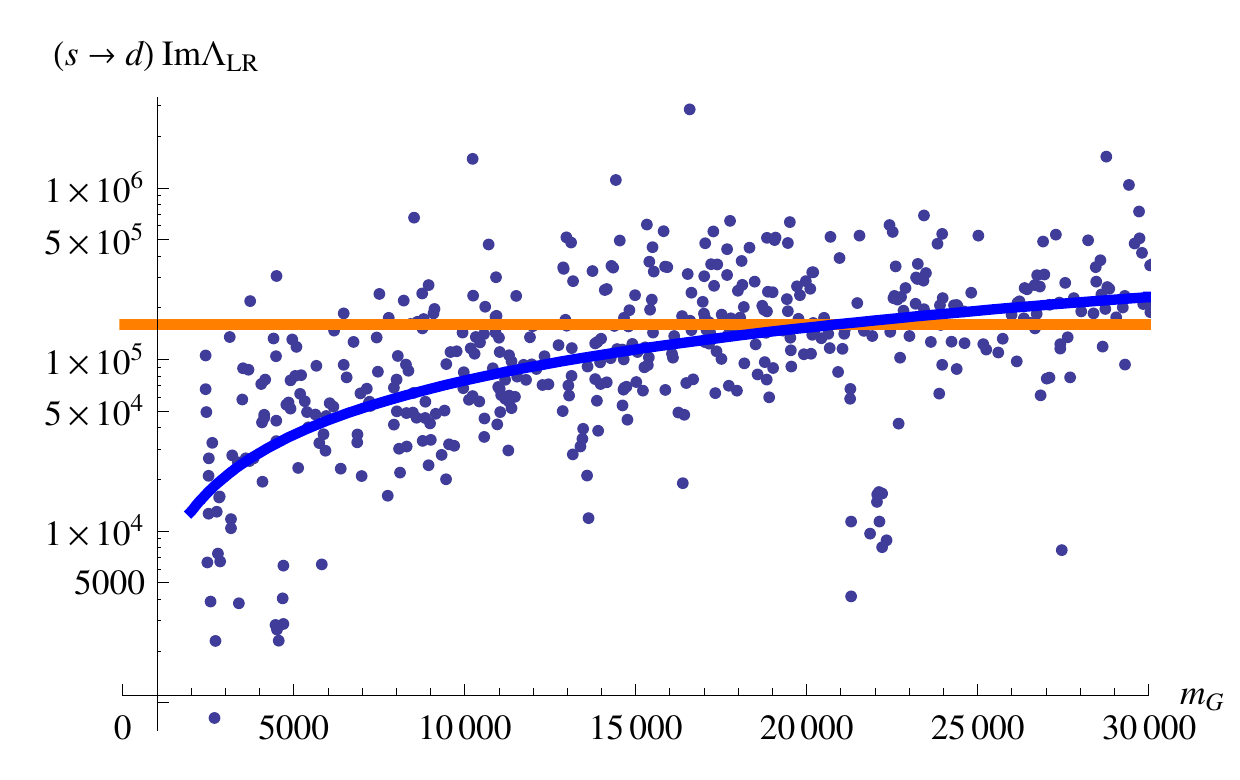
\includegraphics[width=\linewidth]{cfw_fig1_epsK.png}\\[2pt]
{\footnotesize Fig.~1: KK-gluon $\mathrm{Im}\,\Lambda_{LR}$ vs.\ $m_G$; the bound is crossed around $m_G\approx20$~TeV.}
\end{minipage}

% ---------------- Blanke ----------------
\hdr{$\Delta F=2$ Observables and Fine-Tuning with Custodial Protection}
    {Blanke, Buras, Duling, Gori, Weiler}{Blanke et al.}{\arxiv{0809.1073}}
\noindent
\begin{minipage}[t]{0.55\textwidth}
{\small\itshape Formulas taken}\;{\small none.}\\[6pt]
{\small\itshape What the paper computes}\\[4pt]
{\small The full $\Delta F=2$ set \emph{inside} the custodial model. The $\varepsilon_K$ fine-tuning $\Delta_{BG}$ vs.\ $M_{KK}$ gives
\\[4pt]
$\displaystyle M_{KK}\gtrsim 18~\text{TeV}\ (\Delta_{BG}{<}20),\quad 30~\text{TeV}\ (\Delta_{BG}{<}10).$
\\[4pt]
Direct evidence that custodial does not move the flavor bound.}
\end{minipage}\hfill
\begin{minipage}[t]{0.42\textwidth}
\centering
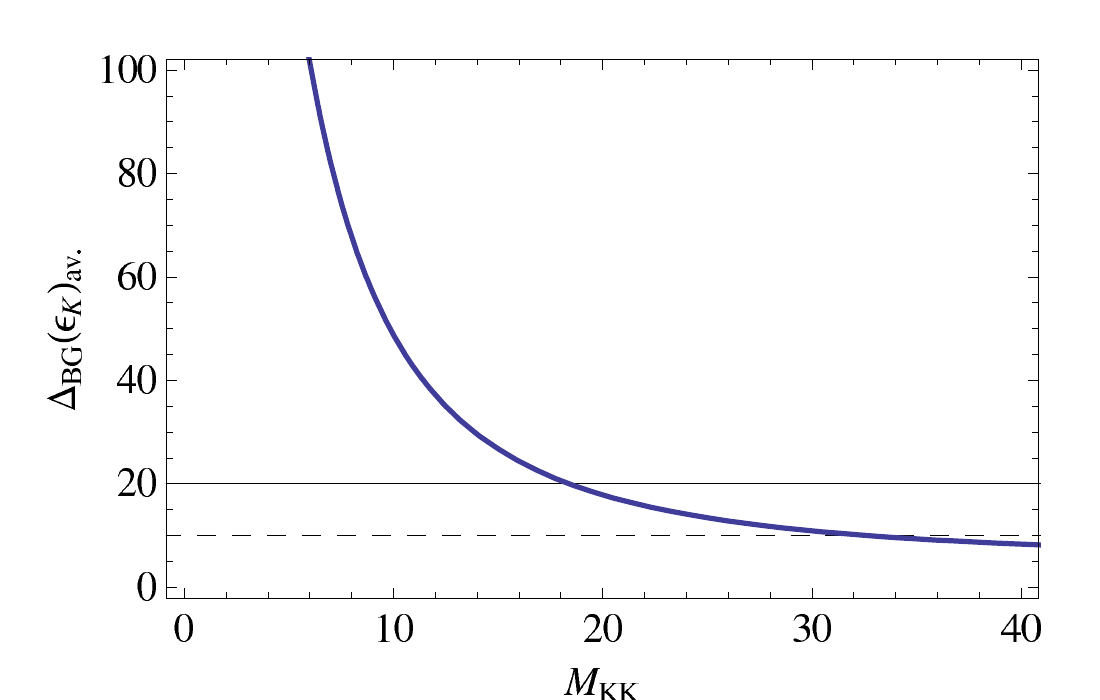
\includegraphics[width=\linewidth]{blanke_fig9_epsK.png}\\[2pt]
{\footnotesize Fig.~9: $\varepsilon_K$ fine-tuning $\Delta_{BG}$ vs.\ $M_{KK}$, computed in the full custodial model. The wall survives custodialization.}
\end{minipage}

% ---------------- Bauer II ----------------
\hdr{Flavor Physics in the Randall-Sundrum Model, II}
    {Bauer, Casagrande, Haisch, Neubert}{Bauer et al., II}{\arxiv{0912.1625}}
\noindent
\begin{minipage}[t]{0.55\textwidth}
{\small\itshape Formulas taken}\;{\small none.}\\[6pt]
{\small\itshape What the paper computes}\\[4pt]
{\small The anarchic minimal $|\varepsilon_K|$ cloud (our Lane~A baseline), $95\%$-quantile floor
\\[4pt]
$\displaystyle M_g^{(1)}\gtrsim 10~\text{TeV (S1)};$
\\[4pt]
$C_4$ is ``a pure QCD effect \dots\ insensitive to the electroweak embedding''; notes $Zb_L$ is removable by custodial.}
\end{minipage}\hfill
\begin{minipage}[t]{0.42\textwidth}
\centering
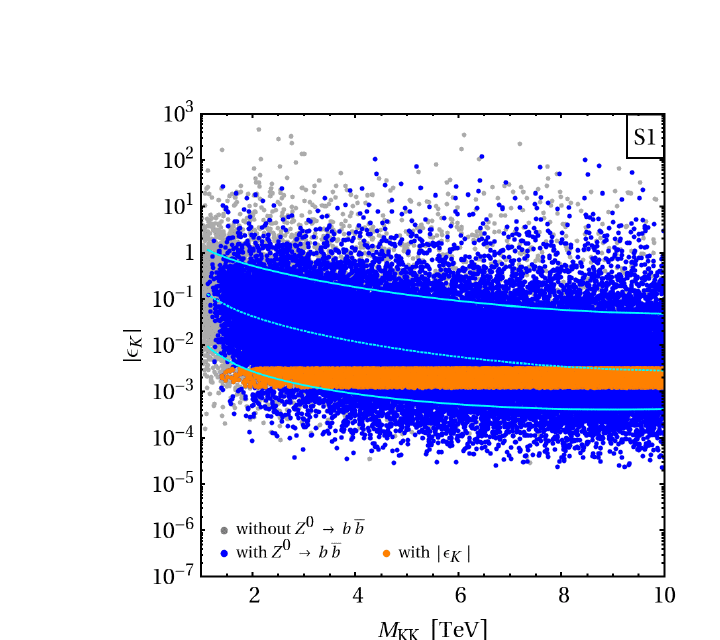
\includegraphics[width=\linewidth]{bauer_fig4_epsK.png}\\[2pt]
{\footnotesize Fig.~4: anarchic $|\varepsilon_K|$ vs.\ $M_{KK}$ (S1), spanning $\sim\!6$ decades; the $95\%$ floor sits near $10$~TeV.}
\end{minipage}

\vspace{1.0em}
\hrule
\vspace{0.5em}
{\small Formulas come from CGHNP, ADMS, ACDP, and CPSW. CFW, Blanke, and Bauer~II supply the comparison figures: custodial protection lowers the electroweak floors for $S,T,U$ and $Z\to b\bar b$ to a few TeV, while the $\varepsilon_K$ wall stays at tens of TeV. Full equation-level provenance (status tags, page numbers, the four proxy gaps) is in \texttt{docs/CUSTODIAL\_PROVENANCE.md}.}

\end{document}
